\documentclass{article}
\usepackage{amsmath,graphicx,tikz,siunitx,url}

\begin{document}
% Structures and text
\section{Introduction}
We write text with special chars: \%, \$, \_, \{ \}, \# and \verb|\texttt{code\_with\_underscores}|.
A URL: \url{https://example.com/?q=\LaTeX}.

\subsection{A Figure}
\begin{figure}
\centering
\fbox{\rule{0pt}{3cm}\rule{4cm}{0pt}} % placeholder box
\caption{A boxed placeholder}
\label{fig:box}
\end{figure}

\subsection{A Table}
\begin{table}
\centering
\begin{tabular}{lcr}
\hline
Left & Center & Right\\
\hline
$\alpha$ & $x^2$ & \SI{3.14}{\metre}\\
\hline
\end{tabular}
\caption{Tiny table}
\label{tab:tiny}
\end{table}

\subsection{TikZ}
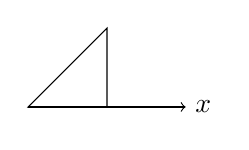
\begin{tikzpicture}
  \draw (0,0) -- (1,0) -- (1,1) -- cycle;
  \draw[->] (0,0) -- (2,0) node[right] {$x$};
\end{tikzpicture}

\subsection{Lists}
\begin{itemize}
  \item First \textbf{bold} and \emph{emph}.
  \item Inline math $a_1, a_2, \dots, a_n$ and display:
  \[
    \sum_{k=0}^{n} r^k = \frac{1-r^{n+1}}{1-r}.
  \]
  \item Command samples: \newcommand{\foo}{bar}, \tikzpicture, \includegraphics, \begin{tabular} etc.
\end{itemize}
\end{document}
